\documentclass[twocolumn,20pt]{article}

\usepackage[english]{babel}
\usepackage[utf8]{inputenc}
\usepackage[T1]{fontenc}
\usepackage{listings}
\usepackage{graphicx}
\usepackage{comment}
\usepackage{amsmath}
\usepackage{hyperref}



\title{Assessed Coursework 2 Report\linebreak Advanced Programming }

\author{Willian de Oliveira Barreiros Junior\\
Matric Number: 2105514\\
 guns945@gmail.com\\}

\begin{document}
\maketitle

\section{Introduction}
This report regards the implementation details of a file crawler to generate a dependency list for the \textit{make} tool on large projects.

The report will be divided into three parts. First, a complete overview of the architecture implemented, second, the thread-safe collections used and, finally, the tests results.

The source code from this coursework can also be found at
\url{https://github.com/WillianJunior/AdvancedProgramming3Project2}

\section{Architecture Overview}
The crawler implementation uses three thread layers, the main layer, or the dispatcher, the workers layer, and the harvest layer, as we can see in figure \ref{fig:arch}.

\begin{figure}[h]
\centering
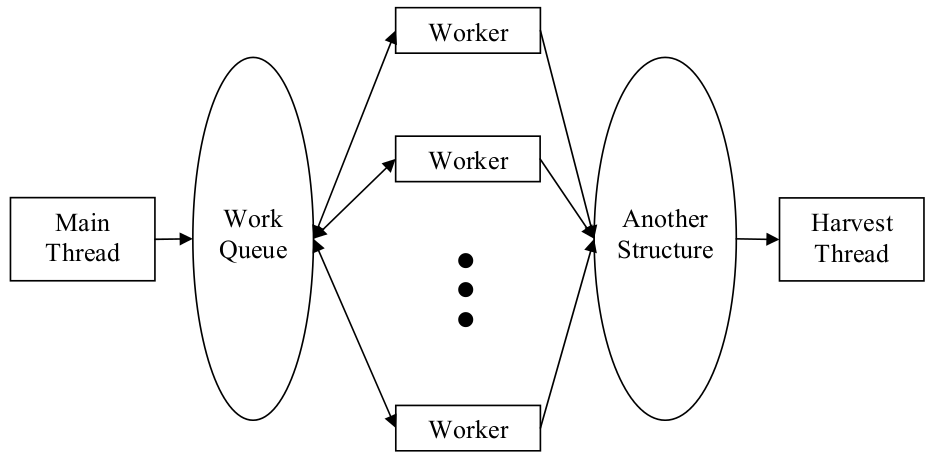
\includegraphics[scale=0.20]{arch.png}
\caption{Required Architecture}
\label{fig:arch}
\end{figure}

\subsection{The Dispatcher}
The main thread has two main goals, generate the shared collections (the work queue is included) and start all other threads. 

The main thread is also responsible for knowing when the crawling is over, and then, finish the execution of the program.

The execution order for the main thread is shown at listing \ref{lst:mainExecOrder}.

\begin{lstlisting}[caption={Main thread execution order}, label=lst:mainExecOrder]
1. Generate directory list
2. Generate work queue
3. Spawn the harvest thread
4. Create the workers thread pool
5. Spawn the worker threads
6. Wait for the end of the worker threads
7. Wait for the end of the harvest thread
\end{lstlisting}

\subsection{The Workers}
Each worker thread keep trying to get an entry from the work queue until the same is empty. When this happens the thread end its execution.

The entry processing is done by making a list of processed dependencies from a first list of dependencies that need to be processed (this beginning with only the name of the file from the work queue). As new dependencies are processed, these are copied to the output list. When there is no more dependencies the processing stop and return the output list.

\subsection{The Harvester}
As soon as the harvest thread begins to run it will try to get the first value from the output list. The output list have a blocking \textit{pop} method, which only returns the first element of the list if it is the expected one (given the ordering). Otherwise the method will block the caller thread until the \textit{add} method is called, on which case will check again if is possible to return the first element.

The harvest thread will keep poping entries from the output list for a predefined number of times. This number is set by the main thread via the harvest's constructor. This way the main thread don't need to signal the harvest thread when all working threads stopped working (as it was implemented in a previous version). Also, the harvest thread will consume the output list as the worker threads are populating it.

\section{Thread-Safe Collections}
The crawler counts with four thread-safe collections, three that are actually used by the threads and one that is a superclass for one of the collections. The shared collections are: the work queue, the directory list and the output list.

All of the mentioned concurrent collections were implemented by encapsulating unsafe existing collections, giving them thread-safe characteristics.

\subsection{Work Queue}
The work queue was implemented by encapsulating a java \textit{TreeMap} collection. The \textit{TreeMap} was chosen since it is an ordered structure, making it easy to get the elements in order. Also, given that the \textit{Map} collection has a key, this was used also at the output list, to order the output.

There are three main methods on this collection:\textit{add}, \textit{pop} and \textit{size}. \textit{Add} insert a new \textit{String} into the \textit{TreeMap} ensuring mutual exclusion between multiple thread access, and also assigning the \textit{Map} elements' ids. \textit{Pop} return the first element in the \textit{Map}, after removing it. \textit{Pop} also ensure mutual exclusion to avoid that more than one working thread process the same entry. \textit{Size} returns the \textit{Map} size. Given the implementation, there is no need for synchronising this method, since only the main thread calls \textit{add} and \textit{size}.

\subsection{Directory List}
The directory list is the most different structure from the three collections used. It implements a sort of lock, that, once locked, there is no way to update the collection contents. All functions related to adding a new element or locking the list are synchronised to make the collection thread-safe.

Unlike the work queue and the output list, the directory list is implemented encapsulating a simple java \textit{List}.

The only way to access the list is through an immutable iterator, being this a read-only iterator. This was thought to improve the concurrency between working threads. Using this implementation there is no need for locks nor synchronisation, but the collections still keeps being thread-safe.

\subsection{Output List}
The final thread-safe collection implemented is the output list. Since this structure needs to be ordered and thread-safe, it extends the collection used by the work queue, making some minor changes.

As it was mentioned before, this collection need to have blocking access, i.e. block the caller thread when is impossible to pop an entry, and wake it up whenever a new entry is added.

The first step is to implement the \textit{blockingPop} method. This will be the one used. Just to make sure that it is impossible to call a non-blocking pop, the \textit{pop} method was overwritten, throwing \textit{UnsupportedOperationException}.

In order to assure that only valid elements are popped out, the container have a key counter to keep track on which is the next element to be popped. When an element is popped the counter increments.

A new \textit{add} method also needs to be implemented, so that whenever there is an insertion the waiting threads may be awakened. Since we are dealing with multiple insertions that are not necessarily in the same order, so, the new \textit{add} needs the entry's id as an input parameter. This id is the same from the work queue, this way ensuring the correct output ordering.

\section{Tests Results}
Two tests were performed: one for correctness and one for performance.
\subsection{Correctness}
The first step to ensure that the crawler is properly working is to check out for deadlocks. This was done by testing repeatedly with over 50 worker threads (50 to 200 threads). There was not a single thread deadlocked on every test.

The next step is to ensure that all the shared structures were being setup properly. This test is a little bit trickier since the only way to ensure that is checking the content of the structures on runtime.

The final step is, of course, test against the handout test instance and compare the result with the expected one.

All correctness test were successful, indicating that the implemented file crawler is fully working (at least for the given test instance) using multiple worker threads.

\subsection{Performance}
To ensure the best possible throughput on a multithread worker-dispatcher program, the number of running threads is a critical factor. In order to identify the best worker threads number the program was tested using 1 to 20 worker threads. Since the worker thread number only affect the time taken from the start of the worker threads to when all of them are finished, that interval will be the only one taken into consideration.

As shown in figure \ref{fig:eff}, after two threads, the increase of the worker threads number is harmful to the program performance. This can mean that either the achieved concurrency wasn't good enough (i.e. most threads locked while only few are really working), or that the instance used for testing wasn't big enough to take advantage of using a large number or worker threads.

\begin{figure}[h]
\centering
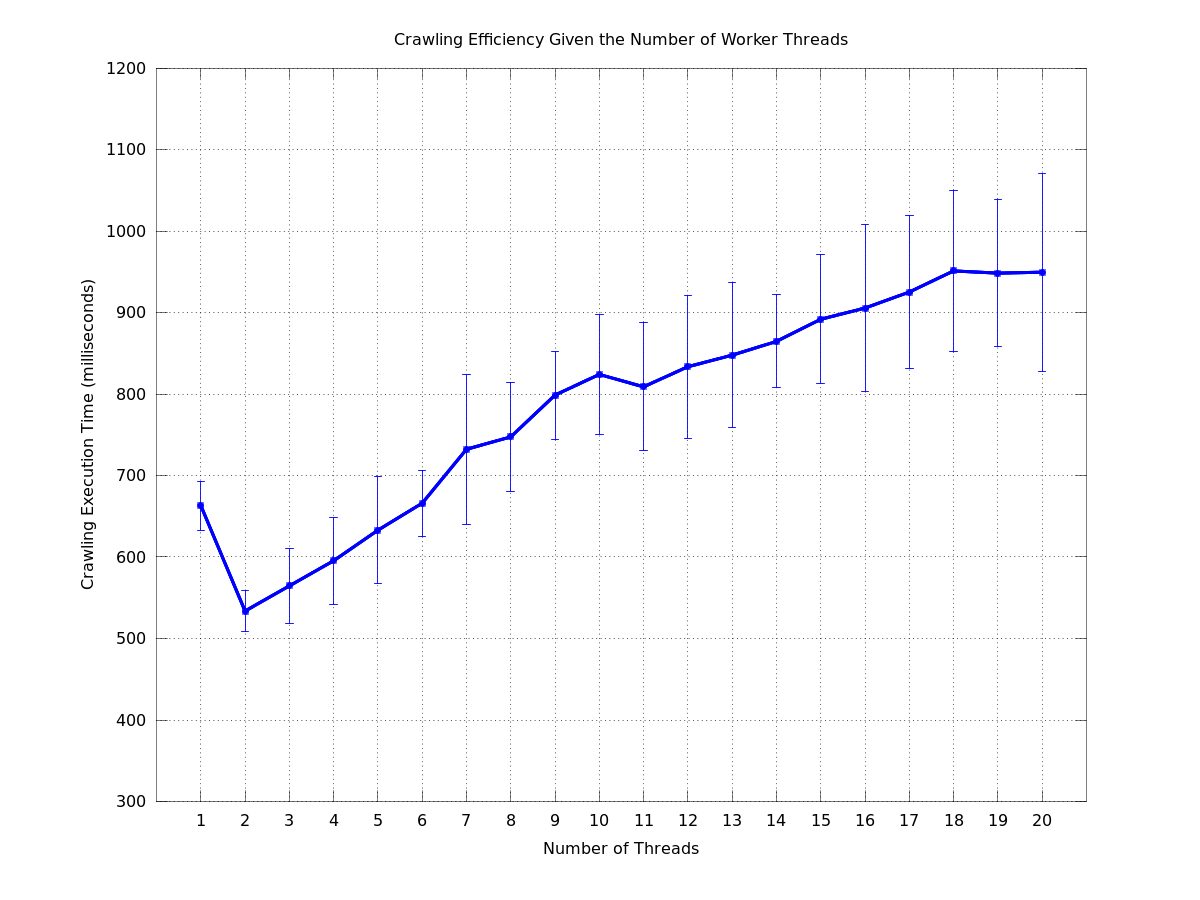
\includegraphics[scale=0.19]{effPerThreadError.png}
\caption{Efficiency of crawling given the number of worker threads}
\label{fig:eff}
\end{figure}

\section{Final Remarks}
Some improvements that can still be done. One is to optimise the spawn rate of worker threads by using the already existent worker threads to help the main thread.

Also we can change the underlying container on the output list, from the current \textit{MapTree} to a simple array. This way no locks would be needed on the output list if we could guarantee that no two threads would be working on the same file (which is already implemented). 

The final improvement that could be done in order to optimise the crawling is to use a new collective collection to store the already processed dependencies (e.g. given that a first file has the dependencies d1.h and d2.h and that there is a second file with the dependencies d2.h and d3.h, the second file would benefit from the execution of the first by just searching the dependency d2.h instead of crawling).

\end{document}
